\section{Experiments and Evaluation}
\label{sec:experiments}

In this section, we evaluate our method on the TU-Berlin sketch benchmark, which is the largest human sketch dataset to date.
%
It contains in total 20000 sketches of 250 categories. Each category has 80 instances.
%
We conducted a group of experiments to compare our method with other methods in both recognition accuracy and number of trainable parameters.
%
We performed three-fold cross validation within the dataset using
the same strategy with previous methods~\cite{Yu2015SketchaNetTB, Dupont2016DeepSketch2D}.
%Like previous works, we use 3-fold cross-validation within the dataset.
Dataset augmentation is also performed to ease the over-fitting problem, same as~\cite{Yu2015SketchaNetTB}.


%\vspace{0.15cm}
\noindent \textbf{Training strategy.}
%
Our SketchPointNet, which is composed of all fully-connected layers, can be trained end-to-end by back-propagation and Adam, with the softmax classification loss.
%
For the multilayer perceptrons in the entire network, we use parameters mlp(8,16,64), mlp(64,16,2) in PN-1, mlp(32,32,128), mlp(128,64,29) in PN-2, mlp(64,128,1024), mlp(512,256,250) in PN-3.
%
However, the entire network is easily converged to a local optima and suffers from over-fitting.
Moreover, the third PointNet PN-3 plays a different role from PN-1 and PN-2. It captures more global pattern for classification.
%
The network parameters are densely distributed in PN-3, which tends to converge on the training set without sufficient training for PN-1 and PN-2.


To solve this problem, we developed a three-step training strategy.
%
We re-initialize parameters randomly in PN-3 to ensure that the parameters in PN-1 and PN-2 are trained sufficiently.
%
In the first step, we randomly initialize all the parameters in the SketchPointNet and train it in an end-to-end fashion.
%
In the second step, we initialize the first two mini PointNets PN-1 and PN-2 for local pattern extraction with the parameters obtained in the first step, and randomly initialize the parameters in the third mini PointNet PN-3. Then we retrain the entire network.
%
In the third step, repeat the second step for three times.
%
Table ~\ref{tbl:iteration} shows the improvement of recognition accuracy with our three-step training strategy.
%, we can see that the recognition results on evaluation dataset are getting higher and higher after numbers of iterations of training. It shows that our training strategy is effective.

\begin{table}[htbp]
\centering
\caption{Recognition accuracy under different training step.}
\label{tbl:iteration}
\begin{tabular}{l|lll}
    \hline
     Training& step 1&  step 2& step 3\\
    \hline
     split 1& 70.8 \% & 73.8\% & 74.3\% \\
     split 2& 71.2\% & 73.6\% & 74.3\% \\
     split 3& 70.8\% & 72.5\% & 74.0\% \\
    \hline
\end{tabular}
\end{table}



\noindent\textbf{Accuracy and Model Size.}
%
We compare our SketchPointNet with state-of-the-art approaches on the TU-Berlin benchmark, considering both the recognition accuracy and model compactness.
%
Comparing with traditional techniques using hand-crafted features, our SketchPointNet performs significantly better.
%
We compare our method with two types of approaches using deep networks.
The first type of methods include Sketch-a-Net~\cite{Yu2015SketchaNetTB}, DeepSketch 1~\cite{Seddati2015DeepSketchDC}, and DeepSketch 2~\cite{Dupont2016DeepSketch2D}.
These methods consider sketches as raster images and use deep convolutional networks as image classification.
The second type includes PointNet++~\cite{qi2017pointnetplusplus}, PointCNN~\cite{1801.07791}, which treat sketches as a set of points.


The comparison is presented in Table~\ref{tb:acc-size}.
As shown, our algorithm achieves comparable performance $74.22\%$ with image-based convolutional networks.
%
Compared to the vanilla version without any fusion part, our SketchPointNet achieves higher performance than Sketch-a-Net~(vanilla)~\cite{Yu2015SketchaNetTB}, and comparable results with DeepSketch 1~\cite{Seddati2015DeepSketchDC}.
However, as designed, our SketchPointNet is very compact by using lots of shared weights.
Ours has about $5$ times less parameters than Sketch-a-Net~(vanilla)~\cite{Yu2015SketchaNetTB} and $30$ times less parameters than DeepSketch 1~\cite{Seddati2015DeepSketchDC}.
%
The models having the highest recognition accuracy ($77.95\%$ for Sketch-a-Net~\cite{Yu2015SketchaNetTB}, and $77.69\%$ for DeepSketch 2~\cite{Dupont2016DeepSketch2D}) both employ a complex fusion step, which makes their network significantly larger.
%
We believe that our method could also be greatly improved in the future by feature fusion.


Compared with the point-based methods (PointNet++~\cite{qi2017pointnetplusplus} and PointCNN~\cite{1801.07791}), our SketchPointNet improves the recognition accuracy by more than $6\%$, without increasing model parameters.
This is mainly because our algorithm considers both temporal and spatial patterns while they focus on the spatial structure only.

\comments{
\begin{table*}
\centering
\begin{tabular}{llll}
    \hline
     models&group parameters& accuracy& stroke order\\
    \hline
     SketchPointNet(mlp(8,16,64), mlp(32,32,128), mlp(64,128,1024))&group1(512*30), group2(256*100)& 73.5\% & y\\
    \hline
     SketchPointNet(mlp(8,16,64), mlp(32,32,128), mlp(64,128,1024))&group1(512*30), group2(256*100)& 69.6\% & n\\
    \hline
     PointNet++(mlp(8,16,64), mlp(32,32,128), mlp(64,128,1024))&group1(512*30), group2(256*100)& 51.2\% &n\\
    \hline
     PointNet++(mlp(64,64,128), mlp(128,128,256), mlp(256,512,1024))&group1(512*64), group2(128*64)& 58.7\% &n\\
    \hline
     PointNet(mlp(64,64,64,128,1024))&-& 46\% &n\\
    \hline
\end{tabular}
\caption{Comparing with PointNet and PointNet++}
\label{tbl:pointnet_cp}
\end{table*}
}


\begin{table}[htbp]
\centering
\caption{Comparison with state-of-the-art results on both recognition accuracy and model compactness.}
\label{tb:acc-size}
%\large
\begin{tabular}{l|rr}
    \hline
     Method & Accuracy & \#Parameters\\
    \hline
  %   HOG-SVM \cite{Eitz2012HowDH}& 56\% & N/A \\
  %   MKL-SVM \cite{LiHSG15} & 65.8\%  & N/A \\
  %   FV-SP \cite{Schneider2014SketchCA} & 68.9\%  & N/A\\
  %   LeNet \cite{LeCun1998GradientbasedLA}& 55.2\%  & N/A\\
  %   \hline
     Sketch-a-Net \cite{Yu2015SketchaNetTB}& 77.95\%  & 8.2M\\
     DeepSketch 2 \cite{Dupont2016DeepSketch2D}& 77.69\%  & 276M\\
     \hline
     DeepSketch 1 \cite{Seddati2015DeepSketchDC}& 75.42\%  & 55.1M\\
     Sketch-a-Net(vallina) \cite{Yu2015SketchaNetTB}& 72.6\% & 8.2M \\
     \hline
     PointNet++ \cite{qi2017pointnetplusplus}& 66.53\%  & 1.73M\\
     PointCNN \cite{1801.07791}& 67.72\%  & 0.89M\\
     \hline
     Ours& 74.22\%  & 1.64M\\
    \hline
\end{tabular}
\end{table}


Fig.~\ref{fig:resshow} shows two groups of examples.
In the top row, the three examples are correctly recognized as their ground-truth categories.
Compared to PointNet, which investigates critical points for each class, our SketchPointNet extracts critical patterns for each category.
%
Take the first sketch as example, the head part is recognized as a panda, though its pose is more like an human. Similarly, SketchPointNet recognizes the second sketch as tiger mainly from the head part and the stripes on its body.
%
Although our network can handle some challenging cases, there are still some challenging cases.
As the bottom row in Fig.~\ref{fig:resshow} shows, the sketches are extremely ambiguous cases.
%, due to the limit of painting skills of non-expert users.

\begin{figure}[htbp]
    \center
    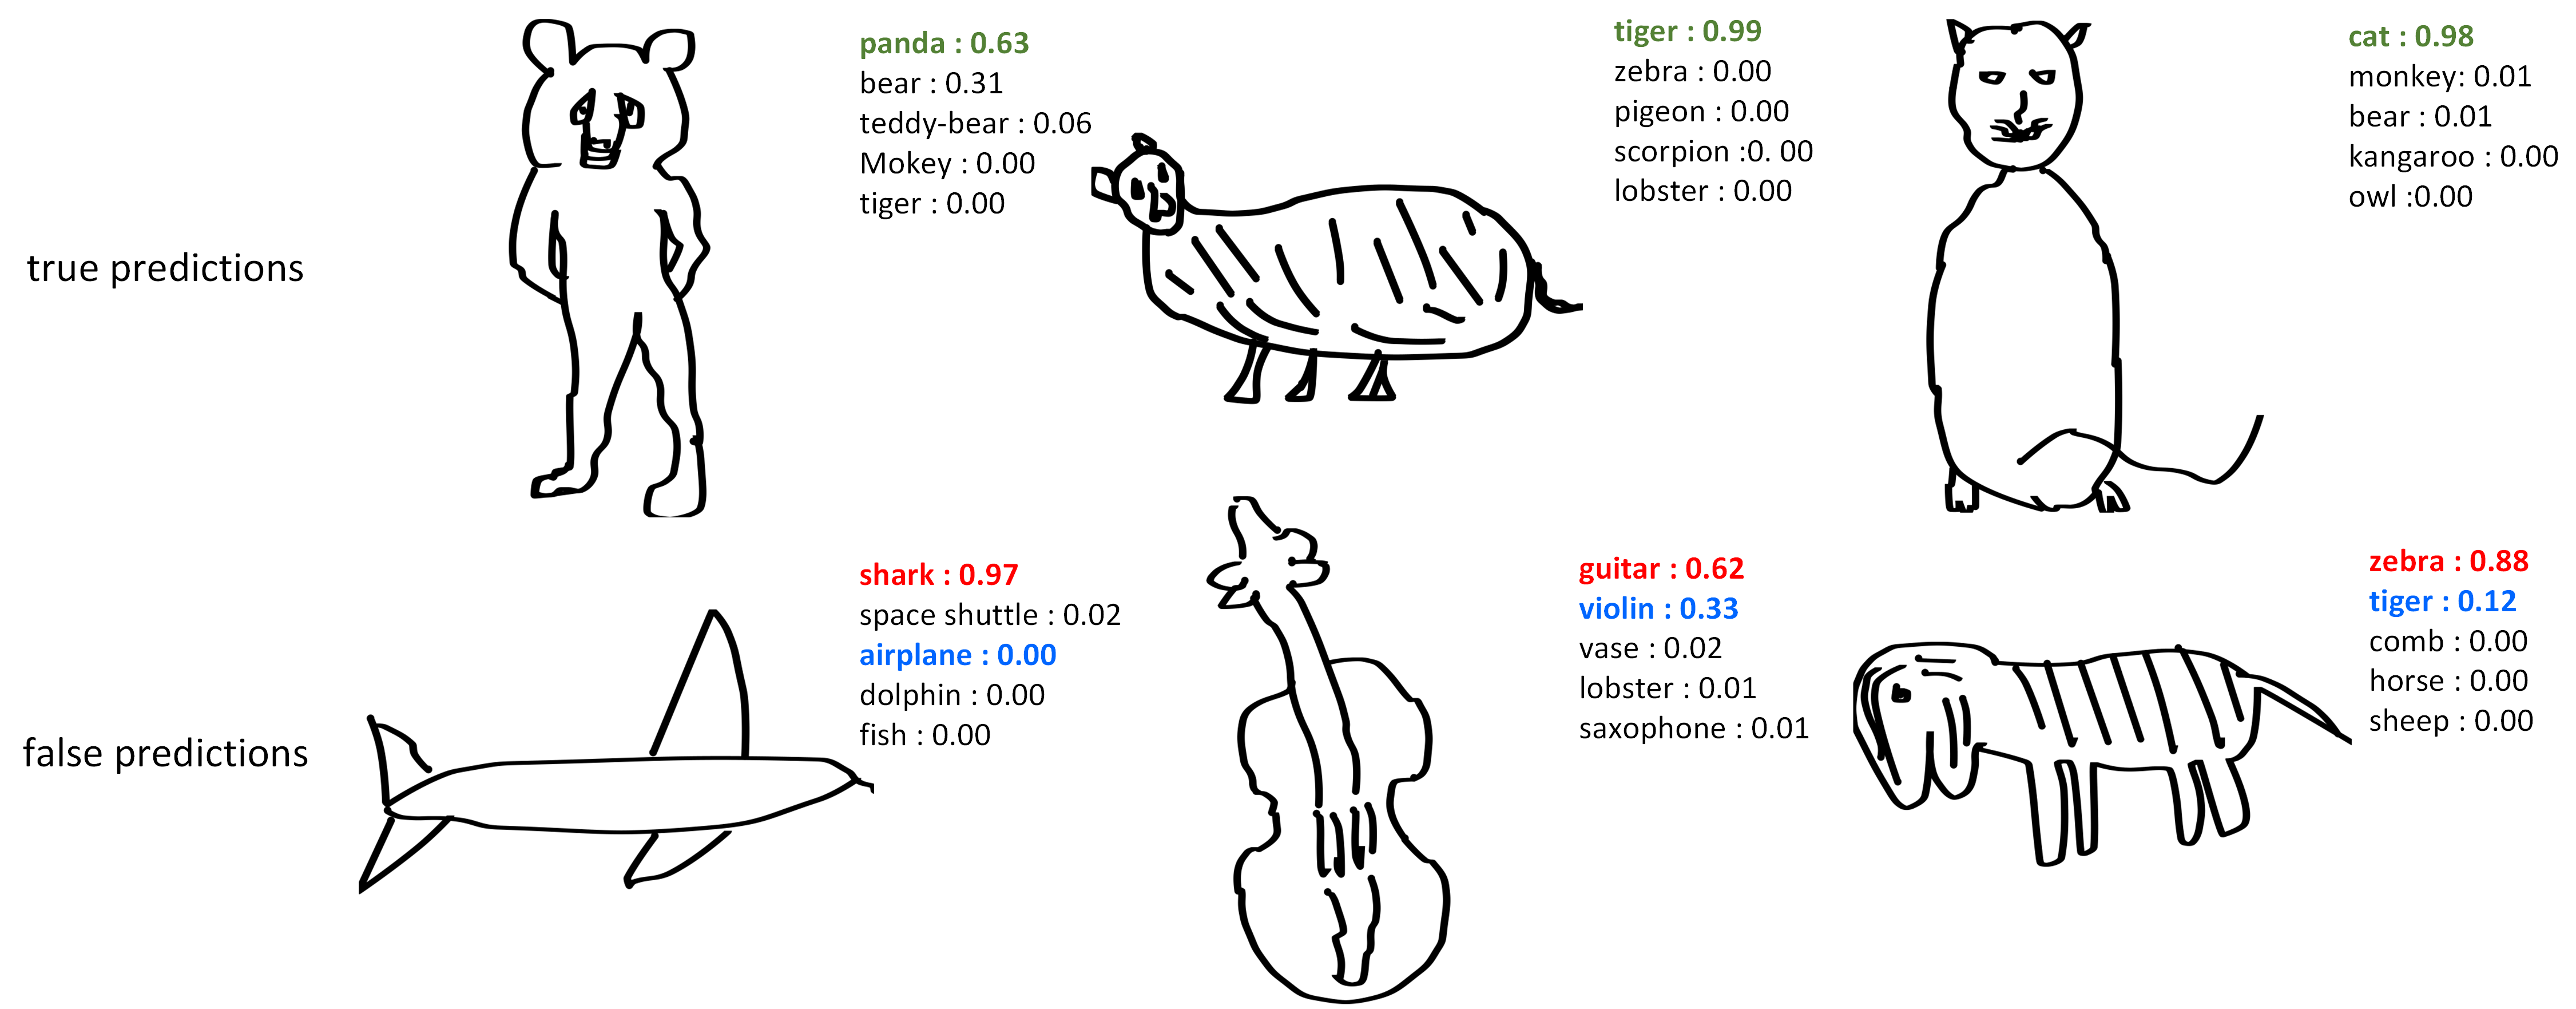
\includegraphics[width=3in]{images/res.png}
    \fcaption{Some easy cases (top row) and challenging cases (bottom row) for SketchPointNet. The green labels indicate correct predictions. The red lables indicate the wrong classification, while the ground-truth categories are shown in blue.  }
    \label{fig:resshow}
\end{figure}
